% ============================================================================
% 4. Simulaciones -- esqueleto fijo, no se edita (solo el orden de los \input).
% Cada subsección vive en su propio fichero, con su responsable.
% ============================================================================
\section{Simulaciones numéricas}
\label{sec:sim}

Los experimentos usan el simulador común \texttt{src/ssm.py}, que integra la EDO de tokens con Runge--Kutta de orden~4 y detecta la explosión en tiempo finito.
Cada script de \texttt{experiments/} guarda sus figuras en \texttt{figures/}.

\subsection{Efecto de la dimensión de estado}
\label{sec:sim-dimension}

\todo{Objetivo: por la observación~\ref{obs:ssm-rango}, $\estado$ solo entra por el rango de $\Mmat$; con $D=1$ no tiene efecto. Se usa $D>1$.}

\paragraph{Diseño.}
Para cada $\estado$ se comparan tres familias de $\Mmat$, con la escala elegida para que $\tr(\Mmat)/D$ no dependa de $\estado$:
\begin{itemize}[nosep]
  \item $\Mmat=-S\transp S$, semidefinida negativa de rango $\estado$ (análogo de $\mu<0$);
  \item $\Mmat=+S\transp S$, semidefinida positiva de rango $\estado$ (análogo de $\mu>0$);
  \item $\Mmat=\SC\transp\SB$ con $\SB,\SC$ independientes (no simétrica, en general indefinida).
\end{itemize}
Cada realización se clasifica como convergente, divergente o intermedia en $t_{\max}$.
\todo{Parámetros usados ($D$, $L$, $t_{\max}$, número de realizaciones, $S_\Delta$, $a$).}

\paragraph{Resultados.}
\begin{figure}[t]
  \centering
  \includegraphics[width=\linewidth]{dimension_estado_trayectorias.png}
  \caption{Norma máxima de los tokens en función de $t$ para distintas dimensiones de estado $\estado$ y las tres familias de $\Mmat$.}
  \label{fig:dim-trayectorias}
\end{figure}

\begin{figure}[t]
  \centering
  \includegraphics[width=0.9\linewidth]{dimension_estado_aleatorio.png}
  \caption{Fracción de realizaciones convergentes, intermedias y divergentes en función de $\estado$, y norma final relativa.}
  \label{fig:dim-aleatorio}
\end{figure}

\todo{Comentar los resultados con los números definitivos (ejecutar con más realizaciones). Conectar con la sección~\ref{sec:din-general}.}

\subsection{Efecto de la parametrización}
\label{sec:sim-param}

\paragraph{Diseño.}
Caso unidimensional. Se barren el signo de $\mu$, el decaimiento $a$ y la escala $S_\Delta$, y se dibuja la norma de cada token frente a $t$ en escala logarítmica.
Usamos $L=6$ tokens y, salvo que se indique lo contrario, $a=1$. Los tres escenarios son:
\begin{itemize}[nosep]
  \item \emph{convergencia}: $\mu=-1$, $S_\Delta=1$, $x(0)=(1,-0.7,0.5,0.9,-1.2,0.6)$ y $t_{\max}=50$;
  \item \emph{divergencia lenta}: $\mu=1$, $S_\Delta=-3$, $x(0)=(0.8,0.9,\dots,1.3)$, de modo que $S_\Delta x_l(0)\le-2.4<-2.12$ y decrece con la posición ($t_{\max}=50$);
  \item \emph{divergencia rápida}: $\mu=1$, $S_\Delta=1$, $x(0)=(0.5,0.7,0.9,1.0,1.1,1.3)$, todos con $S_\Delta x_l(0)>0$ ($t_{\max}=5$).
\end{itemize}
En los barridos se toman $a\in\{0.1,1,5\}$ y $S_\Delta\in\{0.5,1,2,4\}$. La EDO se integra con Runge--Kutta de orden~4 y se declara explosión cuando algún token supera $10^6$.

\begin{figure}[t]
  \centering
  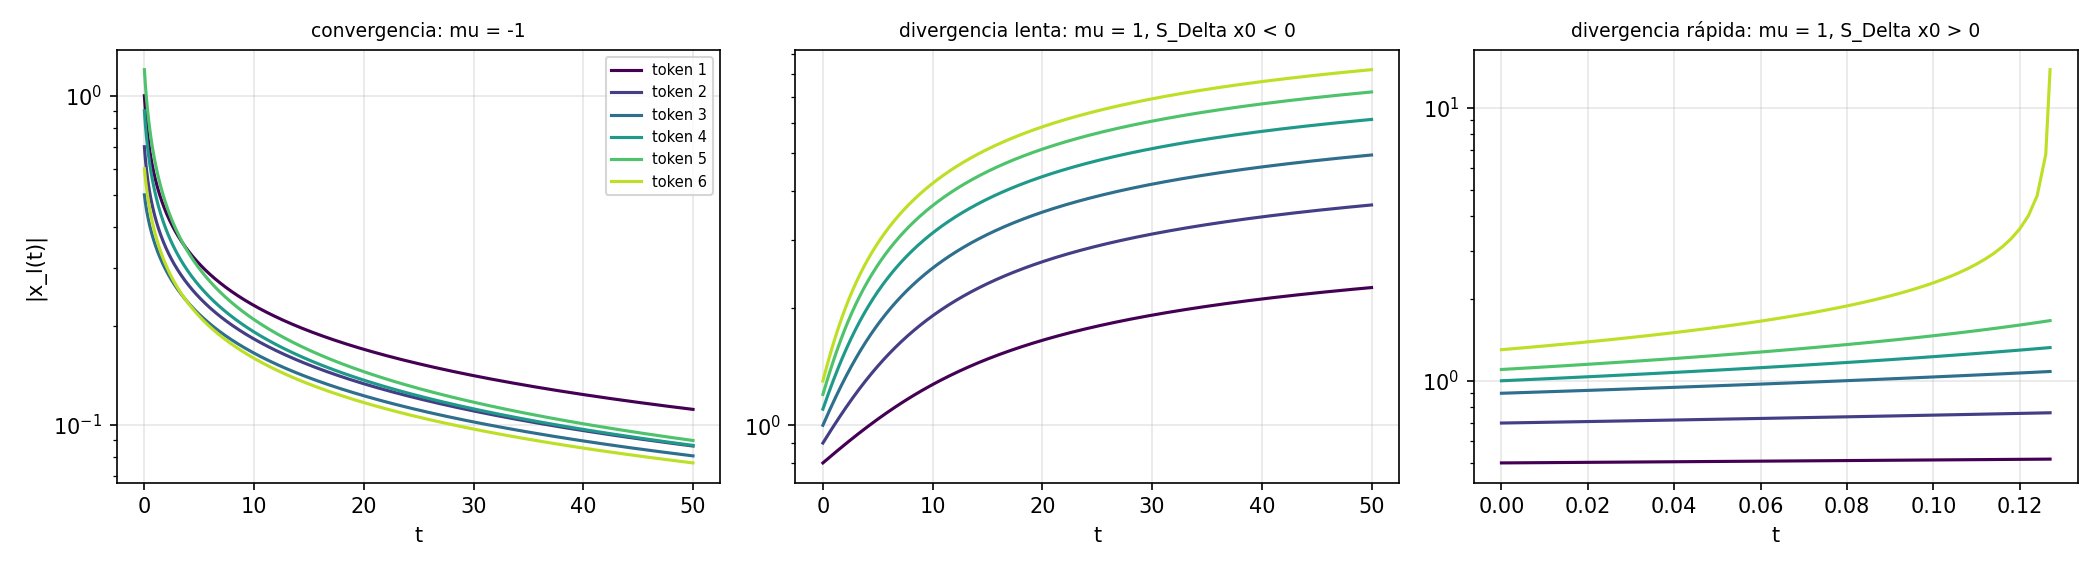
\includegraphics[width=\linewidth]{param_escenarios.png}
  \caption{Los tres escenarios del caso unidimensional: convergencia, divergencia lenta y divergencia rápida.}
  \label{fig:param-escenarios}
\end{figure}

\begin{figure}[t]
  \centering
  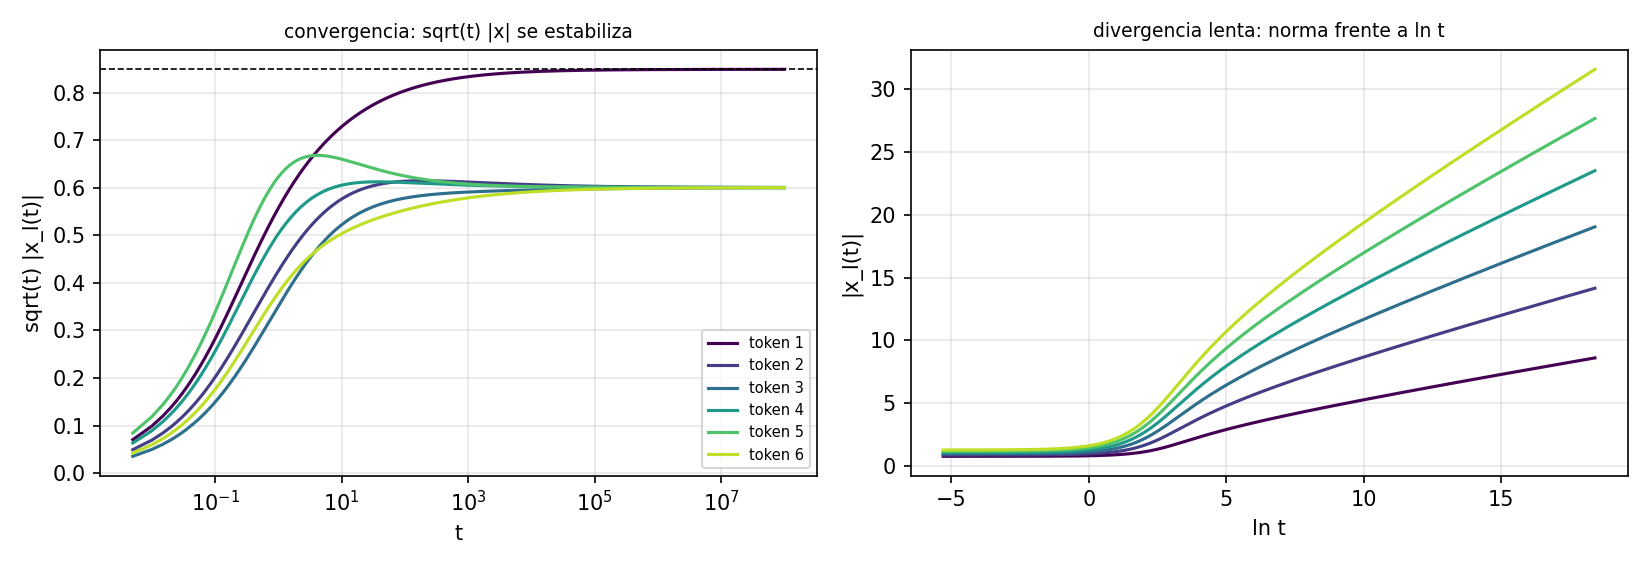
\includegraphics[width=\linewidth]{param_tasas_largas.png}
  \caption{Comprobación de las tasas del teorema a tiempos largos.}
  \label{fig:param-tasas}
\end{figure}

Los tres escenarios coinciden con la clasificación de la sección~\ref{sec:din-1d} (figura~\ref{fig:param-escenarios}). Con $\mu<0$ todos los tokens decaen y a $t=50$ cumplen $\lvert x_l\rvert\in[0.08,0.11]$. Con $\mu>0$ y $S_\Delta x_l(0)\le-2.12$ crecen sin explotar, hasta $\lvert x_l(50)\rvert\approx 2.3,\,3.7,\dots,8.2$ para $l=1,\dots,6$, y el crecimiento aumenta con la posición. Con $S_\Delta x_l(0)>0$ la solución explota en tiempo finito, aquí en $t\approx0.127$.

El parámetro $a$ cambia poco el comportamiento cualitativo (barridos no mostrados en figuras, disponibles en \texttt{figures/}). En convergencia solo desplaza el nivel de los tokens $l\ge2$: con $a=0.1$ valen $0.02$--$0.06$ a $t=50$ y con $a=5$ unos $0.11$--$0.13$, es decir, un $a$ grande aísla los tokens y cada uno evoluciona como si estuviese solo, de forma que su norma tiende a la del primer token ($0.111$). En divergencia lenta apenas hay diferencias ($\lvert x_6(50)\rvert$ pasa de $8.3$ a $7.8$). Algo parecido ocurre con $S_\Delta$ en convergencia: el primer token pasa de $0.115$ a $0.096$ al multiplicar $S_\Delta$ por~8. Ni $a$ ni $S_\Delta$ modifican, por tanto, el escenario; lo fija el signo de $\mu$ y el de $S_\Delta x_l(0)$.

Por último, comprobamos las tasas de la sección~\ref{sec:din-tasas} integrando hasta $t=10^8$ con paso proporcional a $t$ (figura~\ref{fig:param-tasas}). En convergencia la pendiente log-log de $\lvert x_l\rvert$ para $t>10^4$ es $-0.50$ en los seis tokens, igual a la del teorema~\ref{thm:din-conv}. En divergencia lenta, un ajuste $\lvert x_l\rvert\sim(\ln t)^{\beta}$ para $t>10^3$ da $\beta\approx0.8$ en todos los tokens, compatible con la cota $(\ln t)^l$ del teorema~\ref{thm:din-lenta}, que para $l=1$ ya vale $\beta\le1$. La cota no es ajustada para $l>1$: la simulación no muestra la dependencia en $l$ del exponente, aunque sí que el crecimiento es más rápido en los tokens posteriores.

\subsection{Longitud de secuencia y memoria de largo contexto}
\label{sec:sim-long}

\paragraph{Diseño.}
Se mide cuánta memoria del primer token conserva el último al crecer el número de tokens $L$, con dos medidas: el peso $\lvert P_{L1}\rvert$ y la sensibilidad $\lvert\partial x_L(T)/\partial x_1(0)\rvert$ (calculada con el método del paso complejo).
También se estudia cómo cambia el tiempo de explosión de la divergencia rápida con $L$. Se toman $L\in\{2,4,\dots,64\}$ y $a\in\{0.1,1,5\}$, con los parámetros de los tres escenarios anteriores, y se mide en $T=10$ (en la divergencia rápida, al $80\,\%$ del tiempo de explosión).

\begin{figure}[t]
  \centering
  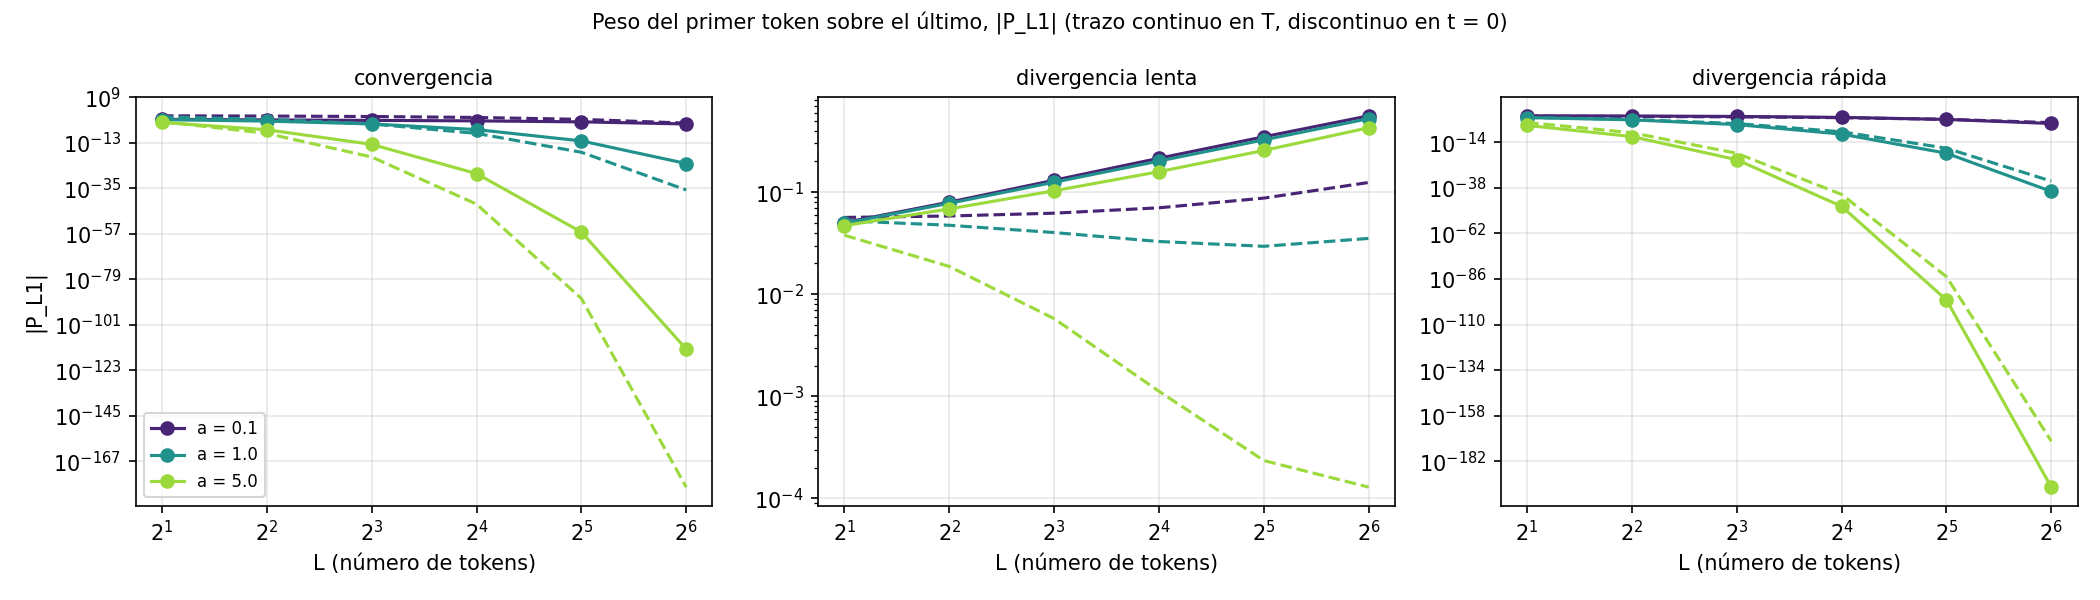
\includegraphics[width=\linewidth]{long_peso.png}
  \caption{Peso del primer token sobre el último, $\lvert P_{L1}\rvert$, frente a $L$.}
  \label{fig:long-peso}
\end{figure}

\begin{figure}[t]
  \centering
  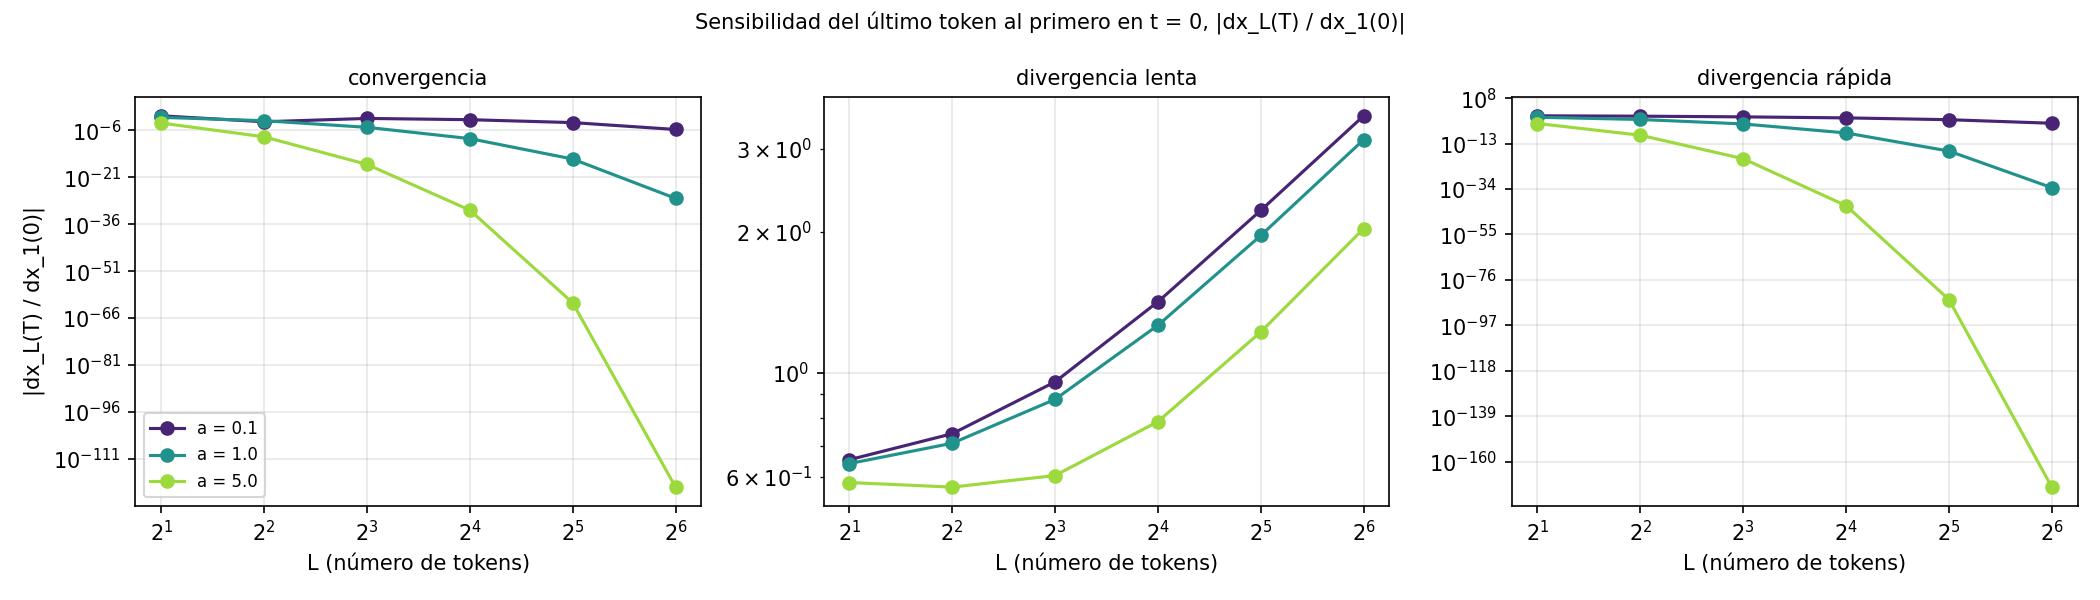
\includegraphics[width=\linewidth]{long_sensibilidad.png}
  \caption{Sensibilidad del último token al primero, $\lvert\partial x_L(T)/\partial x_1(0)\rvert$, frente a $L$.}
  \label{fig:long-sensibilidad}
\end{figure}

\emph{Convergencia.} La memoria se pierde al crecer $L$ y lo hace más deprisa cuanto mayor es $a$. Con $a=1$, la sensibilidad en $T=10$ baja de $1.4\cdot10^{-2}$ ($L=2$) a $2\cdot10^{-28}$ ($L=64$). La causa es el factor $\exp(-a\sum_{k=2}^{L}\Delta(x_k))$ de $P_{L1}$: como $\Delta(x_k)$ no se anula, la suma crece con $L$ (de $0.8$ a $50$ con $L=2,\dots,64$) y el decaimiento es exponencial en la longitud. Incluso con $a=0.1$ la sensibilidad cae de $4\cdot10^{-2}$ a $2\cdot10^{-6}$.

\emph{Divergencia lenta.} Es el único escenario en que el último token conserva información del primero. Los $\Delta(x_k)$ son casi nulos ($S_\Delta x_k\le-2.4$), así que $\sum_k\Delta(x_k)$ satura por debajo de $10^{-2}$ y el factor exponencial queda $\approx1$ para cualquier $L$ y $a$. De ahí que $\lvert P_{L1}\rvert$ en $T=10$ crezca con $L$ (de $0.05$ a $0.5$ con $a=1$) y también la sensibilidad (de $0.64$ a $3.1$). Debe leerse con cuidado: es un resultado a tiempo finito, y el teorema~\ref{thm:din-lenta} da $P_{lj}\to0$ cuando $t\to\infty$, de modo que la memoria es transitoria aunque la sensibilidad siga creciendo.

\emph{Divergencia rápida.} Con $a\ge1$ la memoria se destruye antes que en convergencia ($\lvert P_{L1}\rvert\sim10^{-40}$ con $a=1$ y $L=64$, y $\sim10^{-196}$ con $a=5$), porque aquí $\sum_k\Delta(x_k)\approx 90$ con $L=64$. Con $a=0.1$ decae más despacio, pero sigue siendo pequeña ($8\cdot10^{-5}$). El tiempo de explosión baja con $L$ solo si $a$ es pequeño ($0.13\to0.03$ con $a=0.1$; $0.137\to0.119$ con $a=1$) y es independiente de $L$ ($0.138$) con $a=5$, porque los tokens quedan desacoplados y explota por sí solo el de mayor valor inicial ($1.3$), que es el mismo para todo $L$.

En resumen, en ninguno de los escenarios que entran en la clasificación de la sección~\ref{sec:din-1d} se conserva memoria de largo contexto de forma sostenida: solo la divergencia lenta la mantiene en un horizonte finito.

